\chapter[Object Detection With YOLO]{Object Detection With YOLO}
\markboth{Chap. 1\ \ \enspace Introduction}{Chap 1. Introduction}

\regularsection
\headerregularsection

\updatemylof % to be used with "list of figure divider per chapter" (see PREAMBLE)

\begin{sloppypar} % to suppress overfull box

  %Lorem \index{Lorem} ipsum dolor sit amet, consectetuer adipiscing elit \cite{LIUDIMULYO201767}. Ut purus \index{purus} elit,vestibulum ut, placerat ac, adipiscing vitae, felis \citenum{LIUDIMULYO201767}. Curabitur dictum \index{dictum} gravidamauris. Nam arcu libero, nonummy eget, consectetuer id, vulputate a, magna. Donec vehicula augue eu neque \cite{liudimulyo_2018}. Pellentesque habitant morbi tristique senectuset netus et malesuada fames ac turpis egestas \index{egestas}\citenum{liudimulyo_2018}. Mauris ut leo. Cras viverra metusrhoncus sem \cite{2019liudimulyo}. Nulla et lectus vestibulum urna fringilla ultrices. Phasellus eutellus sit amet tortor gravida placerat \citenum{2019liudimulyo}. Integer sapien est, iaculis in, pretium quis,viverra ac, nunc. Praesent eget sem vel leo ultrices bibendum \cite{liudimulyo2020853}. Aenean faucibus. Morbi dolor nulla, malesuada eu, pulvinar at (\ref{fig:figures/paper-iv/fig-1}), mollis ac, nulla. Curabitur auctorsemper nulla \citenum{liudimulyo2020853}. Donec varius orci eget risus. Duis nibh mi, congue eu, accumsaneleifend, sagittis quis, diam. Duis eget orci sit amet orci dignissim rutrum \cite{LIUDIMULYO201767,liudimulyo_2018,2019liudimulyo,liudimulyo2020853,liudimulyo_unpublished1,liudimulyo_unpublished2}.


  YOLO (You Only Look Once) is a state-of-art algorithm devoted to object detection, as the name
  implies it can predict objects just by looking once to the image in a clever way. YOLO makes the
  prediction by classifying the object and locating it in the image. It uses deep learning and CNN
  techniques to detect objects, and distinguishes itself from its competitors because, as its name
  indicates, it requires to see the image only once, allowing it to be the fastest of all although it
  sacrifices a little accuracy. This speed allows users to easily detect objects in real time in videos
  (up to 30 FPS). In other words, YOLO takes as input value an image and passes through the neural
  network that looks like a CNN and returns a vector of bounding boxes and class prediction. To
  understand  better  how  YOLO  makes  the  prediction  we  will  explain  it  with  an  example  of  an
  image as it can be seen in Figure~\ref{fig:figures/paper/yolo-grid}.

\begin{figure}[H] % \begin{figure} will let LaTeX decide the best figure placement for you ; \begin{figure}[H] for forcing the figure placement here ; in the bottom, \begin{figure}[!b] ; top of the page, \begin{figure}[!t]
  \centering
  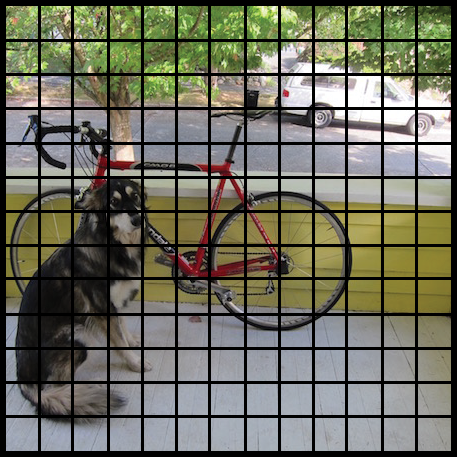
\includegraphics[width=0.60\textwidth]{figures/paper/yolo-grid.png}
  \caption[YOLO divides up the image into a grid of 13 by 13 cells]{YOLO divides up the image into a grid of 13 by 13 cells: Each of these cells is responsible for predicting 5 bounding boxes. A bounding box describes the rectangle that encloses an object.}
  \label{fig:figures/paper/yolo-grid}
\end{figure}


\end{sloppypar}



\section{YOLO in brief}
  To perform de detection YOLO first divides the image into an S x S grid of cells, in Figure~\ref{fig:figures/paper/yolo-grid} we
  can  see  that  the  image  is divided  into  a  13 x  13  grid  of  cells.  In  each of the cells  it  predicts  N
  possible  bounding  boxes  and  calculates  the  level  of  certainty  (probability)  of  each  of  them
  (shown in Figure 13), that is, S x S x N different bounding boxes are calculated in the image, the
  vast majority of them with a very low level of certainty. The score of each BB does not classify
  what type of object is or it does not know what object is fitting the bounding box, it just gives a
  confidence value or a probability value of how good the BB is surrounding an object in each cell.
  In case of Figure~\ref{fig:figures/paper/yolo-grid} for each grid cells 5 bounding boxes are predicted and are graphically shown
  in~\ref{fig:figures/paper/yolo-grid-2} where the higher the probability is the fatter the box is. Each cell makes N bounding
  box predictions and M class probabilities.


  \begin{figure}[H] % \begin{figure} will let LaTeX decide the best figure placement for you ; \begin{figure}[H] for forcing the figure placement here ; in the bottom, \begin{figure}[!b] ; top of the page, \begin{figure}[!t]
  \centering
  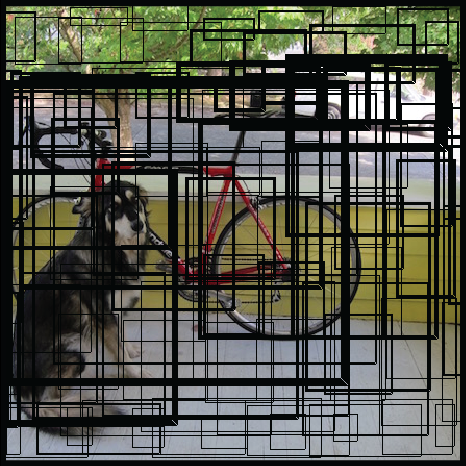
\includegraphics[width=0.60\textwidth]{figures/paper/yolo-grid-2.png}
  \caption[The predicted bounding boxes]{The predicted bounding boxes may look something like this, the higher the confidence score, the fatter the box is drawn}
  \label{fig:figures/paper/yolo-grid-2}
\end{figure}


The bounding box prediction is formed by 5 components: x, y, width, height, confidence score.

\begin{itemize}
\item The (x, y) components are like a mathematical graph coordinates that refer to the centre
of the box, relative to the grid cell location. If the centre of the bounding box does not
fall inside the grid cell this means that the grid cell is not responsible of the object that
has predicted the bounding box. This happens because each object that appears in the
image is related to a single grid cell that is responsible for predicting the object. (x, y)
are normalized between 0 and 1.

\item (Width,  height)  represent  the  dimension  of  the  box  that  contains  an  object,  they  are
also normalized to values from 0 to 1 and they are fundamental to locate the object in
the image.
\item Confidence score  is  a  real value  that  represents  the assurance  the  algorithm  has  that
the box contains an object of any class. The method how the confidence is calculated
will be explained later.

\end{itemize}


\section{The Predictions Vector}
The first step to understanding YOLO is how it encodes its output. The input image is divided into an S x S grid of cells. For each object that is present on the image, one grid cell is said to be “responsible” for predicting it. That is the cell where the center of the object falls into.

Each grid cell predicts B bounding boxes as well as C class probabilities. The bounding box prediction has 5 components: (x, y, w, h, confidence). The (x, y) coordinates represent the center of the box, relative to the grid cell location (remember that, if the center of the box does not fall inside the grid cell, than this cell is not responsible for it). These coordinates are normalized to fall between 0 and 1. The (w, h) box dimensions are also normalized to [0, 1], relative to the image size.


%\section{Section 1 in chapter 1}
%\lipsum[2]

%\begin{equation}
%    EQE = \frac{q \times P_{opt}}{I \times h\nu}
%\end{equation}

%\lipsum[3-4]

%\subsection{Subsection 1.1 of section 1 in chapter 1}
%\lipsum[5-7]

%\subsection{Subsection 1.2 of section 1 in chapter 1}
%\lipsum[8-10]

%\clearpage\phantomsection % to fix wrong hyperref to this section
%\section[Long section title displayed in the table of content]{Short section title in the chapter}
%\sectionmark{Even shorter title on the header}
%\lipsum[11-20]

%\subsection{Subsection 1.2 of section 2 in chapter 1}
%\lipsum[13-14]

%=======================================================================
%%% References

% \clearpage
\phantomsection
\specialsection % put an indent, see preamble
\headerspecialsection

{\hypersetup{urlcolor=ntnu,linkcolor=sophia} % set clickable URL title color to black, not ntnu like in the main document

  \bibliographystyle{unsrtnat-mod}  % NATBIB ref style
  \bibliography{references}
}
